\chapter{Preliminares}
\label{chap:preliminaries}

En este capítulo se presentan las principales definiciones y conceptos que serán usados en el resto del trabajo, además
se analizan los trabajos anteriores que exponen estrategias de solución del problema de la satisfacibilidad
booleana  mediante formalismos de la teoría de lenguajes.

\section{Teoría de Lenguajes}

En esta sección se presentan los principales conceptos de teoría de lenguajes que sirven de base al contenido de los 
capítulos y secciones posteriores, ya que en este trabajo se presentan estrategias para la solución del problema
de la satisfacibilidad empleando mecanismos de la teoría de lenguajes.

\subsection{Conceptos básicos}

Los conceptos básicos de la teoría de lenguajes formales son alfabeto, cadena y lenguaje. Un alfabeto, denotado 
como $\Sigma$, es un conjunto finito y no vacío de símbolos; una cadena es una sucesión finita de símbolos del alfabeto y 
un lenguaje es un conjunto de cadenas definido sobre un alfabeto. Por ejemplo, el 
alfabeto $\Sigma=\{1,0\}$ está formado por los símbolos 0 y 1, $11$ y $101$ son cadenas sobre el alfabeto $\Sigma$ y un ejemplo de lenguaje
es  el conjunto de cadenas de 0 y 1 que terminan en 1.

Dados los conceptos básicos, a continuación se definen operaciones entre alfabetos y cadenas.

\subsection{Operaciones con Lenguajes}

Como los lenguajes son conjuntos, todas las operaciones sobre conjuntos también se definen para lenguajes: unión, intersección, complemento \cite{authomataTheory}.

\paragraph{Homorfismo:} Dados un alfabeto \( \Sigma \) y un alfabeto \( \Gamma \), un homomorfismo es una función:
\[
  h: \Sigma \to \Gamma^*
\]
tal que:
\begin{enumerate}
  \item Para cada \( a \in \Sigma \), \( h(a) \) es una cadena en \( \Gamma^* \).
  \item Si $w=a_1a_2\ldots a_n$ es una cadena entonces
        $$h(w)=h(a_1)h(a_2)\ldots h(a_n).$$
\end{enumerate}

Por ejemplo si sobre el alfabeto $\Sigma=\{a,b\}$, se define el homomorfismo $h$, tal que $h(a)=0$ y $h(b)=11$, entonces
$h(ab)=011$.

Estos conceptos son la base de la teoría de lenguajes y de estos 
se derivan algunas preguntas como determinar si una cadena pertenece a un lenguaje o determinar si un lenguaje es 
vacío. A continuación se presentan 2 problemas que serán usados en el desarrollo de este trabajo, 
el primero se utiliza en los capítulos \ref{chap:LSATFT} y \ref{chap:LSATRCG} y el segundo es utilizado
en \cite{aCFSAT} y \cite{aSRCSAT} (estos trabajos serán descritos más adelante).

\subsection{Problemas relacionados con Lenguajes}

En esta sección se representa el problema de la palabra y el problema del vacío.

\paragraph{Problema de la palabra:} Consiste en determinar si una cadena pertenece a un lenguaje dado.

Por ejemplo dado el lenguaje $L=\{w\,|\,\text{last}(w)=0\}$, $\text{last}(w)$ determinar si $1100100$ pertenece a $L$.

Todo problema en Ciencia de la Computación puede ser reducido a un problema de la palabra, ya que cualquier problema puede ser codificado como un lenguaje formal \cite{authomataTheory}.

\paragraph{Problema del vacío:} Consiste en determinar si un lenguaje es vacío. 
Por ejemplo dado el lenguaje determinar si el conjunto de números pares mayores que 5, que sean primos es vacío.

En la próxima sección se presentan las gramáticas, un mecanismo que permite definir un lenguaje.

\subsection{Gramáticas}

Una \textbf{gramática} es un formalismo utilizado para describir lenguajes formales. Se define como una 4-tupla:
\[
  G = (N, \Sigma, P, S),
\]
donde:
\begin{itemize}
  \item \(N\): Es un conjunto finito de \textbf{símbolos no terminales}, que representan variables o categorías intermedias.
  \item \(\Sigma\): Es un conjunto finito de \textbf{símbolos terminales}, que constituyen el alfabeto del lenguaje. Se cumple que \(N \cap \Sigma = \emptyset\).
  \item \(P\): Es un conjunto finito de \textbf{reglas de producción}, cada una de la forma:
        \[
          \alpha \to \beta, \quad \text{donde } \alpha \in (N \cup \Sigma)^* \wedge \beta \in (N \cup \Sigma)^*.
        \]
  \item \(S\): Es el \textbf{símbolo inicial}, \(S \in N\), que define el punto de partida para derivar cadenas del lenguaje.
\end{itemize}

Una derivación en la gramática consiste en seleccionar una \textbf{regla de producción} $\alpha \to \beta$ y sustituir una ocurrencia de 
$\alpha$ en una cadena $w$ por $\beta$.

Una cadena $w$, $w\in\Sigma^*$,  se puede generar por la gramática $G$ si existe una secuencia de derivaciones que comienza con $S$
y termina con la cadena $w$.

El lenguaje generado por una gramática \(G\) se denota como:
\[
  L(G) = \{ w \in \Sigma^* \mid S \overset{*}{\to} w \},
\]
donde \(\overset{*}{\to}\) indica una derivación en cero o más pasos.

A continuación se presenta la jerarquía de Chomsky, que clasifica a los lenguajes formales de acuerdo con su poder de generación.

\subsection{Jerarquía de Chomsky}

La \textbf{Jerarquía de Chomsky} (Figura~\ref{fig:ChomskySchema}) clasifica los lenguajes en cuatro tipos, según las restricciones en sus reglas de producción y la capacidad expresiva de los lenguajes que generan \cite{geeksforgeeks_chomsky_hierarchy}.

\begin{enumerate}
  \item \textbf{Tipo 0: Gramáticas irrestrictas}
        \begin{itemize}
          \item No tienen restricciones en las reglas de producción.
          \item Cada regla tiene la forma: \(\alpha \to \beta\), donde \(\alpha, \beta \in (N \cup \Sigma)^*\) y \(\alpha \neq \varepsilon\).
          \item Todo lenguaje generado por una gramática irrestricta se denomina \textbf{lenguaje recursivamente enumerable}.
        \end{itemize}
        
  \item \textbf{Tipo 1: Gramáticas dependientes del contexto}
        \begin{itemize}
          \item Cada regla tiene la forma: \(\alpha A \gamma \to \alpha \beta \gamma\), donde \(A \in N\), \(\alpha, \beta, \gamma \in (N \cup \Sigma)^*\), y \(|\beta| \geq 1\).
          \item Todo lenguaje generado por una gramática dependiente del contexto se denomina \textbf{lenguaje dependiente del contexto}.
          \item Todo lenguaje dependiente del contexto es también un lenguaje recursivamente enumerable.
        \end{itemize}
        
  \item \textbf{Tipo 2: Gramáticas libres del contexto}
        \begin{itemize}
          \item Cada regla tiene la forma: \(A \to \beta\), donde \(A \in N\) y \(\beta \in (N \cup \Sigma)^*\).
          \item Todo lenguaje generado por una gramática libre del contexto se denomina \textbf{lenguaje libre del contexto}.
          \item Todo lenguaje libre del contexto es también un lenguaje dependiente del contexto.
        \end{itemize}
        
  \item \textbf{Tipo 3: Gramáticas regulares}
        \begin{itemize}
          \item Las reglas tienen la forma:
                \[
                  A \to aB \quad \text{o} \quad A \to a,
                \]
                donde \(A, B \in N\) y \(a \in \Sigma\).
          \item Todo lenguaje generado por una gramática regular se denomina \textbf{lenguaje regular}.
          \item Todo lenguaje regular es un lenguaje libre del contexto.
        \end{itemize}
\end{enumerate}


\begin{figure}
  \centering
  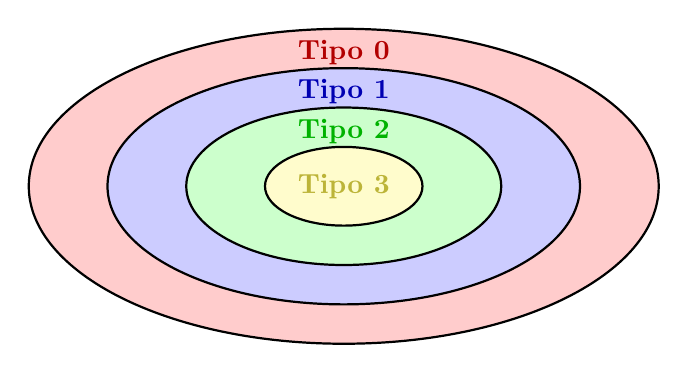
\begin{tikzpicture}[scale=1]
    \draw[thick, fill=red!20] (0,0) ellipse (4cm and 2cm);
    \node at (0,1.7) {\textbf{\textcolor{red!70!black}{Tipo 0}}};
    
    \draw[thick, fill=blue!20] (0,0) ellipse (3cm and 1.5cm);
    \node at (0,1.2) {\textbf{\textcolor{blue!70!black}{Tipo 1}}};
    
    \draw[thick, fill=green!20] (0,0) ellipse (2cm and 1cm);
    \node at (0,0.7) {\textbf{\textcolor{green!70!black}{Tipo 2}}};
    
    \draw[thick, fill=yellow!20] (0,0) ellipse (1cm and 0.5cm);
    \node at (0,0) {\textbf{\textcolor{yellow!70!black}{Tipo 3}}};
  \end{tikzpicture}
  \caption{Esquema de la Jerarquía de Chomsky}
  \label{fig:ChomskySchema} %
\end{figure}

Las diferencias entre los elementos de las jerarquía de Chomsky se pueden ilustrar con el lenguaje \textit{Copy} sobre un alfabeto 
$\Sigma$, que se define como $L_{copy}=\{w^+\,|\,w\in Z^*\}$.  
Si se toma un caso particular de $L_{copy}$, al cual se le llama $L_{copy}^n=\{w^n\,|\,w\in Z^*\}$ y 
el lenguaje $L_{rev-copy}=\{ww_r\,|\,w\in Z^*\}$, donde $w_r$ es $w$ invertida. Se cumple que $L_{copy}^1$
es un lenguaje regular, mientras que $L_{rev-copy}$ es un lenguaje libre del contexto y por último 
$L_{copy}^k\,\forall\,k\geq 2$ es un lenguaje dependiente del contexto \cite{authomataTheory}.  
El lenguaje $L_{copy}$ se usa en los restantes capítulos como base de formalismos que describen el 
lenguaje de las fórmulas booleanas satisfacibles.

En la próxima sección se presentan los principales conceptos relacionados con los autómatas regulares,
los cuales son usados en \cite{aCFSAT} para describir un mecanismo que determina si una asignación
de valores de las variables satisface una fórmula booleana y en el capítulo \ref{chap:LSATFT} se utiliza una extensión
de los autómatas regulares que permite para una asignación de valores de las variables generar todas las fórmulas
booleanas satisfacibles por dichos valores.

\section{Autómatas}
Un autómata es una máquina abstracta que procesa cadenas de símbolos de un alfabeto finito y determina si una 
cadena pertenece a un lenguaje \cite{authomataTheory}.  En esta sección se presentan los 
principales conceptos sobre los autómatas regulares.
\subsection{Autómata regular}

Un autómata regular \cite{authomataTheory}, también conocido como autómata finito, es un modelo matemático que 
permite reconocer si una cadena pertenece a un lenguaje regular y se define como una 5-tupla $$\mathcal{A} = (Q, \Sigma, \delta, q_0, F),$$ donde:

\begin{itemize}
  \item $Q$: Es un conjunto finito de \textbf{estados}.
  \item $\Sigma$: Es el \textbf{alfabeto} finito de entrada.
  \item $\delta$: Es la \textbf{función de transición}, $\delta: Q \times \Sigma \to Q$, que define cómo el autómata cambia de estado en función del símbolo leído.
  \item $q_0 \in Q$: Es el \textbf{estado inicial} desde donde comienza la computación.
  \item $F \subseteq Q$: Es el conjunto de \textbf{estados de aceptación o estados finales}.
\end{itemize}

El autómata comienza en el estado inicial $q_0$ y procede a leer el primer símbolo de la cadena.
En cada paso, la función de transición $\delta$ determina, con base en el símbolo actual de la cadena, el siguiente estado al que debe pasar el autómata, avanzando al siguiente símbolo.
Si, al finalizar la lectura del último símbolo de la cadena, el autómata se encuentra en un estado de aceptación 
$q \in F$, entonces la cadena se acepta; en caso contrario, se rechaza.

Se puede extender el concepto de autómata finito añadiendo un nuevo tipo de transición que no consume ningún caracter, 
la cual recibe el nombre de transición $\varepsilon$. Se puede demostrar \cite{authomataTheory} que el 
conjunto de lenguajes que reconoce un autómata finito sin transiciones $\varepsilon$
(\textit{autómata finito determinista}) es equivalente al conjunto de lenguajes que reconoce 
un autómata finito con transiciones $\varepsilon$ (\textit{autómata finito no determinista}).

A continuación se presenta una extensión de los autómatas finitos, que es usada en el
capítulo \ref{chap:LSATFT} para dada una asignación de valores de las variables, generar todas las fórmulas
booleanas satisfacibles por dichos valores..

\subsection{Transductor finito}

Un transductor finito \cite{finite_transducer} es un modelo computacional que extiende 
los autómatas finitos al incluir una salida para cada transición.  

Formalmente, un transductor finito es un autómata finito con una función de transición extendida que recibe 
un símbolo de la cadena de entrada y un estado, y devuelve el estado al cual pasa el transductor y un símbolo. 
Como resultado de la aceptación de una cadena el transductor genera una cadena de salida formada por todos los 
símbolos que se obtuvieron como resultado mediante la función de transición en el proceso de reconocimiento.

Un transductor finito se define como una 6-tupla:
\[
  T = (Q, \Sigma, \Gamma, \delta, q_0, F),
\]
donde:
\begin{itemize}
  \item \(Q\) es el conjunto finito de estados.
  \item \(\Sigma\) es el alfabeto de entrada.
  \item \(\Gamma\) es el alfabeto de salida.
  \item \(\delta: Q \times \Sigma \to Q \times \Gamma^*\) es la función de transición, que mapea una combinación de estado actual y símbolo de entrada a un nuevo estado y una salida.
  \item \(q_0 \in Q\) es el estado inicial.
  \item \(F \subseteq Q\) es el conjunto de estados finales.
\end{itemize}

Por ejemplo se puede definir el siguiente transductor finito $T$, el cual reconoce cadenas del alfabeto $\{a,b\}$
que tengan ninguna o más $a$ seguida de una o más $b$ y genere una cadena formada por una cantidad de $0$ igual
a la cantidad de $a$ de la cadena original seguida de una cantidad de $1$ igual a la cantidad de $b$ de
la cadena original:
\[
  T = (Q, \Sigma, \Gamma, \delta, q_0, F),
\]
donde:
\begin{itemize}
  \item \(Q = \{q_0, q_1, q_2\}\) es el conjunto de estados.
  \item \(\Sigma = \{a, b\}\) es el alfabeto de entrada.
  \item \(\Gamma = \{0, 1\}\) es el alfabeto de salida.
  \item \(\delta\) es la función de transición definida por:
        \[
          \begin{array}{c|c|c}
            \delta & a        & b        \\
            \hline
            q_0    & (q_0, 0) & (q_1, 1) \\
            q_1    & (q_2, 0) & (q_1, 1) \\
            q_2    & (q_2, 0) & (q_2, 1) \\
          \end{array}
        \]
  \item \(q_0\) es el estado inicial.
  \item \(F = \{q_1\}\) es el conjunto de estados finales.
\end{itemize}

Para reconocer $aaaabbbbb$, primero $T$ empieza por el estado $q_0$ y el primer caracter $a$, entonces pasa al estado $q_0$ y genera un $0$.
Luego, al leer el segundo caracter $a$, se mantiene en el estado $q_0$ y genera otro $0$. Este proceso se repite hasta el quinto caracter
que es $b$, entonces pasa al estado $q_1$. Luego, al leer el sexto caracter $b$, se mantiene en el estado $q_1$ y genera un $1$. Este proceso
se repite varias veces hasta que se llega al final de la cadena, por tanto se genera la cadena $000011111$.

Un homomorfismo es un transductor finito de un solo estado y tantas transiciones hacia el mismo estado como transformaciones de símbolos en el homomorfismo.

Seguidamente se presenta otra máquina abstracta, la cual representa el modelo de cómputo más general de la teoría de lenguajes y 
representa la formalización de un Algoritmo.


\section{Máquina de Turing}

Una Máquina de Turing \cite{authomataTheory} es un modelo abstracto de computación universal introducido por 
Alan Turing en 1936. Este modelo consiste en los siguientes componentes: una cinta, un cabezal de escritura/lectura,
un conjunto de estados y una función de transición.

Una cinta es un medio de almacenamiento infinito dividido en celdas, donde cada celda contiene un símbolo de un alfabeto finito.
Un cabezal de lectura/escritura es un dispositivo que puede leer el contenido de una celda, escribir un nuevo símbolo y moverse a la izquierda o derecha.
El conjunto de estados es colección finita de estados internos que describen la configuración actual de la máquina.
La función de transición es un conjunto de reglas que determinan cómo la máquina cambia de estado, escribe en la cinta y mueve el cabezal en función del estado actual y el símbolo leído.

A continuación de presentan los conceptos de máquina de Turing determinista y máquina de Turing no determinista.

\paragraph{Máquina de Turing determinista (\textit{DTM}):}
En una Máquina de Turing determinista, para cada estado y cada símbolo que se lee, se define como
máximo una transición posible.
\paragraph{Máquina de Turing no determinista (\textit{NTM}):}
En una Máquina de Turing no determinista, para cada estado y símbolo que se lee, pueden existir múltiples transiciones posibles.

Todas las operaciones con lenguajes y los problemas relacionados con ellos tienen una dificultad y para medir esta dificultad
se utiliza un marco teórico llamado complejidad computacional, el cual se presenta en la próxima sección.

\section{Complejidad computacional}

En esta sección se definen los principales conceptos de complejidad computacional: notación asintótica
y las clases de problemas. A continuación se presenta una notación para describir el tiempo que demora un 
algoritmo en realizar determinado cómputo.

\subsection{Notación asintótica}

La notación asintótica se utiliza para describir el comportamiento de una función $f(n)$ a medida que $n$ crece hacia el infinito. 
A continuación se define la notación que será utilizada en el resto del trabajo:

\paragraph{Notación $O(f(n))$}: Una función $g(n)$ pertenece a $O(f(n))$ si existen constantes positivas $c$ y $n_0$ tales que:
\[
  g(n) \leq c \cdot f(n) \quad \text{para todo } n \geq n_0.
\]
Esta notación proporciona un límite superior asintótico para $g(n)$.

La notación asintótica permite describir el tiempo de ejecución de un algoritmo con respecto al número de 
operaciones básicas realizadas por un modelo formal de cómputo (por ejemplo una máquina de Turing). 
Algoritmos como determinar el mínimo y el máximo de un arreglo son $O(n)$, ya que necesitan realizar 
una cantidad $n$ de operaciones básicas en relación con la cantidad de elementos del arreglo.

Se dice que un algoritmo tiene un tiempo polinomial si puede resolverse en una complejidad de $O(n^k)$, donde $n$ es el tamaño de la entrada del algoritmo y $k$
es una constante. Por ejemplo encontrar el mínimo y el máximo de un arreglo tiene un tiempo polinomial, ya que se necesita realizar una cantidad de operaciones
proporcional al tamaño del arreglo.

En la próxima sección se presenta la clasificación de los problemas de acuerdo a su complejidad computacional.
\subsection{Clases de problemas}

Los problemas computacionales \cite{authomataTheory} se agrupan en diferentes clases según los recursos necesarios para resolverlos.

\paragraph{Problemas en la clase P:}
Un problema pertenece a la clase P si puede resolverse en tiempo polinomial. En términos de teoría de lenguajes un lenguaje
$L$ pertenece a P si existe una Máquina de Turing determinista que reconozca $L$ en un tiempo polinomial.

\paragraph{Problemas en la clase NP:}
Un problema pertenece a NP si su solución puede verificarse en tiempo polinomial mediante una Máquina de Turing determinista. Alternativamente, un problema está en NP si puede resolverse en tiempo polinomial mediante una Máquina de Turing no determinista \cite{authomataTheory}.

\paragraph{Problemas en la clase NP-Completo:}
Un problema pertenece a la clase NP-Completo, si pertenece a NP y además es tan difícil como cualquier otro problema en NP. Esto significa que cualquier problema en NP puede reducirse a este problema en tiempo polinómico \cite{authomataTheory}.

\paragraph{Problemas en la clase NP-Duro:}
Un problema pertenece a la clase NP-Duro, si es tan difícil como cualquier otro problema en NP, pero no
necesariamente pertenece a NP \cite{authomataTheory}.

\paragraph{Problemas no decidibles:}
Un problema es no decidible si no existe una Máquina de Turing que pueda resolverlo correctamente para todas las entradas posibles. Esto significa que no hay algoritmo que garantice una respuesta en tiempo finito en todos los casos \cite{authomataTheory}. Un ejemplo clásico de problema no decidible es el \textit{Problema de la Parada} \cite{authomataTheory}, que consiste en determinar si una Máquina de Turing se detendrá para una entrada dada. 

En la siguiente sección se realiza la comparación entre las clases P y NP.

\subsection{P vs NP}

La relación entre las clases P y NP es uno de los problemas abiertos más importantes en la teoría de la
computación \cite{authomataTheory}. Hasta la fecha, se desconoce si $\text{P} = \text{NP}$ o si $\text{P} \neq \text{NP}$,
es decir no se conoce si realmente los problemas en NP son más difíciles que los problemas en P. Por otro
lado el conjunto de problemas NP-Completo brinda una base sólida para el problema anterior, ya que dada su
definición, cualquier problema perteneciente a este conjunto que sea soluble en tiempo polinomial
implica que todos los problemas en NP lo son. Mientras que los problemas en NP-Duro pueden resultar aún más
difíciles. Es decir aunque resultara que $\text{P} = \text{NP}$ no se puede asegurar que no existan problemas
en NP-Duro que no se puedan resolver en tiempo polinomial \cite{authomataTheory}.

Por otra parte existen problemas para los cuales no existe ningún algoritmo, como los problemas indecidibles.

A continuación se presenta el problema que sirve de base a los problemas de la clase NP-Completo: el problema de las satisfacibilidad
booleana.

\section{Problema de la satisfacibilidad booleana}

El problema de la satisfacibilidad booleana (\textit{SAT}), es un problema fundamental en la teoría de la 
computación y la lógica matemática \cite{authomataTheory}. El objetivo es determinar si existe una asignación 
de valores a las variables de una fórmula booleana tal que la expresión sea verdadera.

A continuación se presentan los principales elementos del SAT:

\begin{itemize}
  \item \textbf{Variables booleanas:}
        Una variable booleana es una variable que puede tomar uno de dos valores posibles: \textit{true} (verdadero) o \textit{false} (falso). Estas variables se utilizan para construir expresiones lógicas.
  \item \textbf{Literales:}
        Un literal es una variable booleana o su negación. Formalmente, si \( x \) es una variable booleana, entonces \( x \) y \( \neg x \) (la negación de \( x \)) son literales. Un literal puede tomar los valores \( true \) o \( false \) dependiendo de la asignación de valores a las variables.
  \item  \textbf{Cláusulas:}
        Una cláusula es una disyunción (operador \textbf{OR}) de uno o más literales. Por ejemplo, la cláusula \( (x \vee \neg y \vee z) \) es una disyunción de tres literales: \( x \), \( \neg y \) y \( z \). Una cláusula es verdadera si al menos uno de sus literales es verdadero. Si todos los literales son falsos, la cláusula será falsa.
  \item \textbf{Fórmulas en forma normal conjuntiva:}
        Una fórmula booleana en forma normal conjuntiva (\textit{CNF}) es una conjunción (operador \textbf{AND}) de cláusulas. En otras palabras, es una expresión booleana que se puede escribir como una serie de cláusulas unidas por el operador \textbf{AND}. Por ejemplo:        
        \[
          (x \vee \neg y \vee z) \wedge (\neg x \vee y) \wedge (x \vee \neg z)
        \]
  \item \textbf{Fórmulas booleanas equivalentes:}
        Dos fórmulas booleanas se consideran equivalentes si, para cualquier asignación de valores a sus variables, ambas producen el mismo resultado lógico. Por ejemplo, las fórmulas \( x \vee (y \wedge z) \) y \( (x \vee y) \wedge (x \vee z) \) son equivalentes, ya que para cualquier combinación de valores \( x, y, z \), ambas tienen el mismo valor lógico.
        
        Para cualquier fórmula booleana existe una fórmula booleana equivalente en CNF \cite{authomataTheory} y 
        el algoritmo para encontrarla es polinomial, por lo tanto se puede asumir que toda fórmula booleana está en CNF.
        
\end{itemize}

En la próxima sección define el problema de la satisfacibilidad booleana.

\subsection{Definición del problema de la satisfacibilidad booleana}

El problema de la satisfacibilidad booleana, o SAT, consiste en determinar si existe una asignación de valores \( true \) o \( false \) a las variables de una fórmula booleana tal que la fórmula completa sea verdadera. En términos formales, dado un conjunto de cláusulas en CNF, el problema es encontrar una asignación de valores a las variables que haga que la conjunción de las cláusulas sea verdadera.

Formalmente, se dice que una fórmula booleana en CNF es satisfacible si existe una asignación de valores a las variables tal que todas las cláusulas de la fórmula sean verdaderas simultáneamente.

\begin{itemize}
  \item Si existe tal asignación, la fórmula es \textit{satisfacible}.
  \item Si no existe tal asignación, la fórmula es \textit{insatisfacible}.
\end{itemize}

Un SAT con exactamente $n$ variables distintas en cada cláusula se denomina $n$-SAT.
\subsection{SAT como Problema NP-Completo}

El SAT es el primer problema demostrado como NP-Completo \cite{authomataTheory} y juega un rol central en la teoría de la complejidad computacional. Se define en la clase NP porque, dada una asignación de valores a las variables de la fórmula booleana, se puede verificar en tiempo polinómico si dicha asignación satisface la fórmula.

Además, la prueba de que SAT es NP-Completo fue una de las contribuciones principales de Stephen Cook en 1971 \cite{authomataTheory}, marcando el inicio de la teoría de la NP-completitud.

\subsection{Equivalencia entre SAT y 3-SAT}

Para el problema 2-SAT existe una solución polinomial que determina si la fórmula booleana es satisfacible o no \cite{2satbib}, pero para el problema 3-SAT no se conoce ningún algoritmo polinomial que permita
determinar si una fórmula booleana es satisfacible o no \cite{authomataTheory}.

Cualquier fórmula booleana del problema $n$-SAT se puede reducir a una fórmula booleana equivalente del problema 3-SAT, 
por lo tanto, SAT es equivalente a 3-SAT en términos de complejidad computacional \cite{authomataTheory}.

\subsection{Problemas SAT solubles en tiempo polinomial}

Como se mencionó anteriormente no se conoce ningún algoritmo polinomial para resolver el problema SAT en general, pero
existen casos particulares del problema que sí pueden ser resueltos en tiempo polinomial. A continuación se presentan los
principales casos:

\begin{itemize}
  \item \textbf{1-SAT:} El problema 1-SAT es una instancia particular de SAT donde cada cláusula tiene a lo sumo un literal.
        Este problema puede ser resuelto en tiempo polinomial mediante un algoritmo de asignación de valores de booleanos.
        
  \item \textbf{2-SAT:} El problema 2-SAT es una instancia de SAT donde cada cláusula contiene exactamente dos literales.
        Este problema puede ser resuelto en tiempo polinomial mediante una modelación basada en grafos, 
        utilizando algoritmos como la detección de componentes fuertemente conexas en el grafo de implicación.
        
  \item \textbf{Horn-SAT:} El problema Horn-SAT es una generalización del problema SAT,
        donde cada cláusula tiene a lo sumo un literal positivo. 
        Este problema puede ser resuelto en tiempo polinomial mediante el algoritmo de resolución de Horn.
        
  \item \textbf{XOR-SAT:} El problema XOR-SAT es una instancia de SAT donde cada cláusula representa una operación XOR
        sobre los literales. Puede ser resuelto en tiempo polinomial transformando el problema en un sistema de ecuaciones 
        lineales modulares y aplicando eliminación de Gauss.
\end{itemize}

En la siguiente sección se describen 2 trabajos que vinculan el SAT con la teoría de lenguajes.

\section{Solución de instancias del SAT usando Teoría de Lenguajes}

Como parte del estudio del problema SAT, se han desarrollado anteriormente en 
la Facultad de Matemática y Computación de la Universidad de La Habana 
2 trabajos utilizando un enfoque 
basado en formalismos de la teoría de lenguajes, buscando resolver 
instancias específicas del SAT, que tienen una solución polinomial. 

La idea principal que se aborda en \cite{aCFSAT} consta de tres partes: asumir que todas las variables en 
la fórmula son distintas, construir un autómata finito que reconozca cadenas de 0 y 1 hagan verdadera esa 
fórmula (asumiendo que todas las variables son distintas), y por último intersectar ese lenguaje con algún 
formalismo que garantice que todas las instancias de la misma variable tenga el mismo valor. Luego de esos 
tres pasos, se obtiene un lenguaje libre del contexto de las cadenas de 0 y 1 que satisfacen la fórmula y 
que además respeta los valores de las variables duplicadas.  Finalmente, para determinar si la fórmula es 
satisfacible o no, basta con determinar si el lenguaje es vacío. Todo el algoritmo descrito anteriormente tiene un tiempo polinomial en relación con el 
tamaño de la fórmula booleana.

El autómata finito diseñado en \cite{aCFSAT}, se denominó \textbf{autómata booleano}. La idea detrás de este es representar 
las reglas de la lógica proposicional en transiciones entre los estados de un autómata finito, donde cada estado del autómata representa un valor de verdad positivo o 
negativo lo cual significa que hasta ese momento (solo tomando las instancias de las variables asociadas a los 
caracteres reconocidos) la fórmula se evalúa positiva o negativa respectivamente \cite{aCFSAT}.

Posteriormente en \cite{aCFSAT} se define el concepto del orden libre del contexto: una fórmula booleana tiene un orden libre del contexto si para cualquier par de instancias de una variable $x_i$ y $x_j$ con $i<j$ se
cumple que si existe otra variable con instancia $x_k$ con $i<k<j$ entonces todas las instancias de esta nueva
variable ocurren entre $x_i$ y $x_j$.

Para terminar con lo expuesto en \cite{aCFSAT}, para determinar si una fórmula booleana con un orden libre del contexto 
es satisfacible se intersecta el autómata booleano asociado a dicha fórmula con una gramática libre del contexto 
que comprueba que todas las instancias de las variables tienen el mismo valor, luego se comprueba si el lenguaje
generado es no vacío.

El trabajo expuesto en \cite{aSRCSAT} es una generalización de la idea de \cite{aCFSAT}, pero esta vez se intersecta
el autómata booleano asociado a la fórmula booleana con una gramática de concatenación de rango simple (esta gramática
se define en el próximo capítulo) que describe el orden de las variables. Luego se procede igual que en \cite{aCFSAT}
y se comprueba si el lenguaje generado es no vacío.

En este trabajo se sigue otro enfoque para resolver el SAT usando teoría de lenguajes, en vez de usar el problema del vacío se 
construye el lenguaje de todas las fórmulas booleanas satisfacibles y para determinar si un SAT es satisfacible 
se analiza el problema del vacío. Esto permite demostrar que muchos formalismos tienen el problema de la palabra 
NP-Duro (los que sean cerrados bajo transducción finita 
y además que genere un lenguaje que es subconjunto de $L_{copy}$, el cual se define en el capítulo 
\ref{chap:LSATFT}). Por otro lado se obtiene una gramática de concatenación de rango que reconoce las fórmulas 
booleanas satisfacibles, lo que permite demostrar que las gramáticas de concatenación de rango reconocen todos 
los problemas que pertenecen a la clase NP. Pero antes de esto es necesario definir y analizar las gramáticas 
de concatenación de rango y a ello se dedica el próximo capítulo.